%==============================================================================
% Sjabloon poster bachproef
%==============================================================================
% Gebaseerd op document class `a0poster' door Gerlinde Kettl en Matthias Weiser
% Aangepast voor gebruik aan HOGENT door Jens Buysse en Bert Van Vreckem

\documentclass[a0,portrait]{hogent-poster}

% Info over de opleiding
\course{Bachelorproef}
\studyprogramme{toegepaste informatica}
\academicyear{2023-2024}
\institution{Hogeschool Gent, Valentin Vaerwyckweg 1, 9000 Gent}

% Info over de bachelorproef
\title{Lokaal uitvoeren van Machine Learning pipelines: een vergelijkende studie en Proof of Concept.}
%\subtitle{Ondertitel (eventueel)}
\author{Casper Audenaert}
\email{casper.audenaert@student.hogent.be}
\supervisor{Dhr. S. Lievens}
\cosupervisor{Dhr. T. Aelbrecht (HOGENT)}

% Indien ingevuld, wordt deze informatie toegevoegd aan het einde van de
% abstract. Zet in commentaar als je dit niet wilt.
\specialisation{AI \& Data Engineering}
\keywords{cloud, CI/CD pipelines, machine learning operations, Kubeflow}
\projectrepo{https://github.com/user/repo}

\begin{document}

\maketitle

\begin{abstract}
  Dit onderzoek richt zich op het verkennen van de mogelijkheden voor het lokaal uitvoeren van machine learning pipelines, aan de hand van verschillende frameworks.
  Binnen het keuzepakket ``AI \& Data Engineering'' en het bijbehorende opleidingsonderdeel ``Machine Learning Operations'' wordt er momenteel gebruik gemaakt van Azure ML pipelines voor het uitvoeren van machine learning pipelines in de Azure Cloud.
  Het gebruik van Azure ML pipelines is echter niet gratis voor studenten die niet voldoende krediet hebben op het platform. Hierdoor richt dit onderzoek zich op het lokaal uitvoeren van machine learning pipelines.\\\\
  De basis van Azure ML pipelines is Kubeflow. Voor het lokaal draaien van Kubeflow zijn er echter aanzienlijke uitdagingen, waardoor het noodzakelijk is om een aangepaste Proof of Concept (PoC) op te stellen.
  Het lokaal uitvoeren van machine learning pipelines kan ook problemen met zich meebrengen, zoals de noodzaak van aanzienlijke rekenkracht die mogelijks niet beschikbaar is op computers van studenten. Als gevolg daarvan hebben bepaalde frameworks een beperktere versie die niet zo krachtig is als hun cloud-varianten, maar toch lokaal machine learning pipelines kan uitvoeren.\\\\
  De eerste fase van deze bachelorproef omvat een uitgebreide literatuurstudie waarin onderzocht wordt welke frameworks bestaan voor het lokaal draaien van machine learning pipelines, hoe deze frameworks functioneren, en ook de compatibiliteit en de diverse functies ervan.
  Het tweede deel van dit onderzoek richt zich op het opzetten van een Proof of Concept voor de geselecteerde tool(s), mogelijks vertrekkende van publiek beschikbare manifest bestanden. Hierbij wordt specifiek aandacht besteed aan het gemak van onderhoud voor de betrokken lectoren.
  Het onderzoek leidde tot een aanbeveling voor Prefect, met een grondig begrip van de geschiktheid van diverse frameworks voor het lokaal uitvoeren van machine learning pipelines. Deze aanbeveling biedt praktische toepasbaarheid voor zowel onderwijs als bedrijfsleven.
\end{abstract}

\begin{multicols}{2} % This is how many columns your poster will be broken into, a portrait poster is generally split into 2 columns

\section{Introductie}


Om gebruik te kunnen maken van de Azure-servers hebben gebruikers credits nodig. Tijdens de eerder genoemde opdracht waren er studenten die voor aanvang of tijdens de opdracht geen credits meer hadden. Dit leidde ertoe dat deze studenten hun resultaten niet konden presenteren of zelfs niet konden beginnen aan de opdracht. Daarom wordt in dit onderzoeksvoorstel gekeken naar het opzetten van een lokale installatie van een machine learning-pipeline.
De gekozen frameworks van de shortlist zullen worden gebruikt om verschillende proof of concepts op te stellen. Hierna wordt er gekeken naar hoe elk framework werkt en of het echt wel voldoet aan de vooraf besproken requirements.


\section{Proof of Concepts}
De short list bevatte 3 verschillende frameworks genaamd:
\begin{itemize}
  \item Prefect
  \item ZenML
  \item Dagster
\end{itemize}

Prefect werd gekozen omdat dit framework de meeste functies had en de laagste leercurve van alle frameworks. Vervolgens werd ZenML gekozen omdat dit het nieuwste framework op de longlist was. Hoewel het nog in ontwikkeling is, is het zeer veelbelovend. Ten slotte werd er voor Dagster gekozen omdat dit framework al het langst bestaat en de documentatie goed is uitgewerkt.

Elke Proof of Concept legt uit hoe dat de installatie te werk gaat van de frameworks en hoe dat de pipeline gemaakt kan worden uitgevoerd met dit framework.

\section{Bijhouden van variablen}

Voor het bijhouden van verschillende variabelen wordt MLflow gebruikt. Dit komt voor in elke proof of concept en wordt extern verbonden met elkaar. Dit zorgt ervoor dat de volledige installatie lokaal blijft, zowel het framework als MLflow.

De variabelen die MLflow bijhoudt voor dit onderzoek zijn als volgt:
\begin{itemize}
  \item Eigenschappen van het model
  \item De prestaties van het trainen en evalueren van het model
  \item Systeemeigenschappen tijdens het uitvoeren van een pipeline
\end{itemize}

\begin{center}
  \captionsetup{type=figure}
  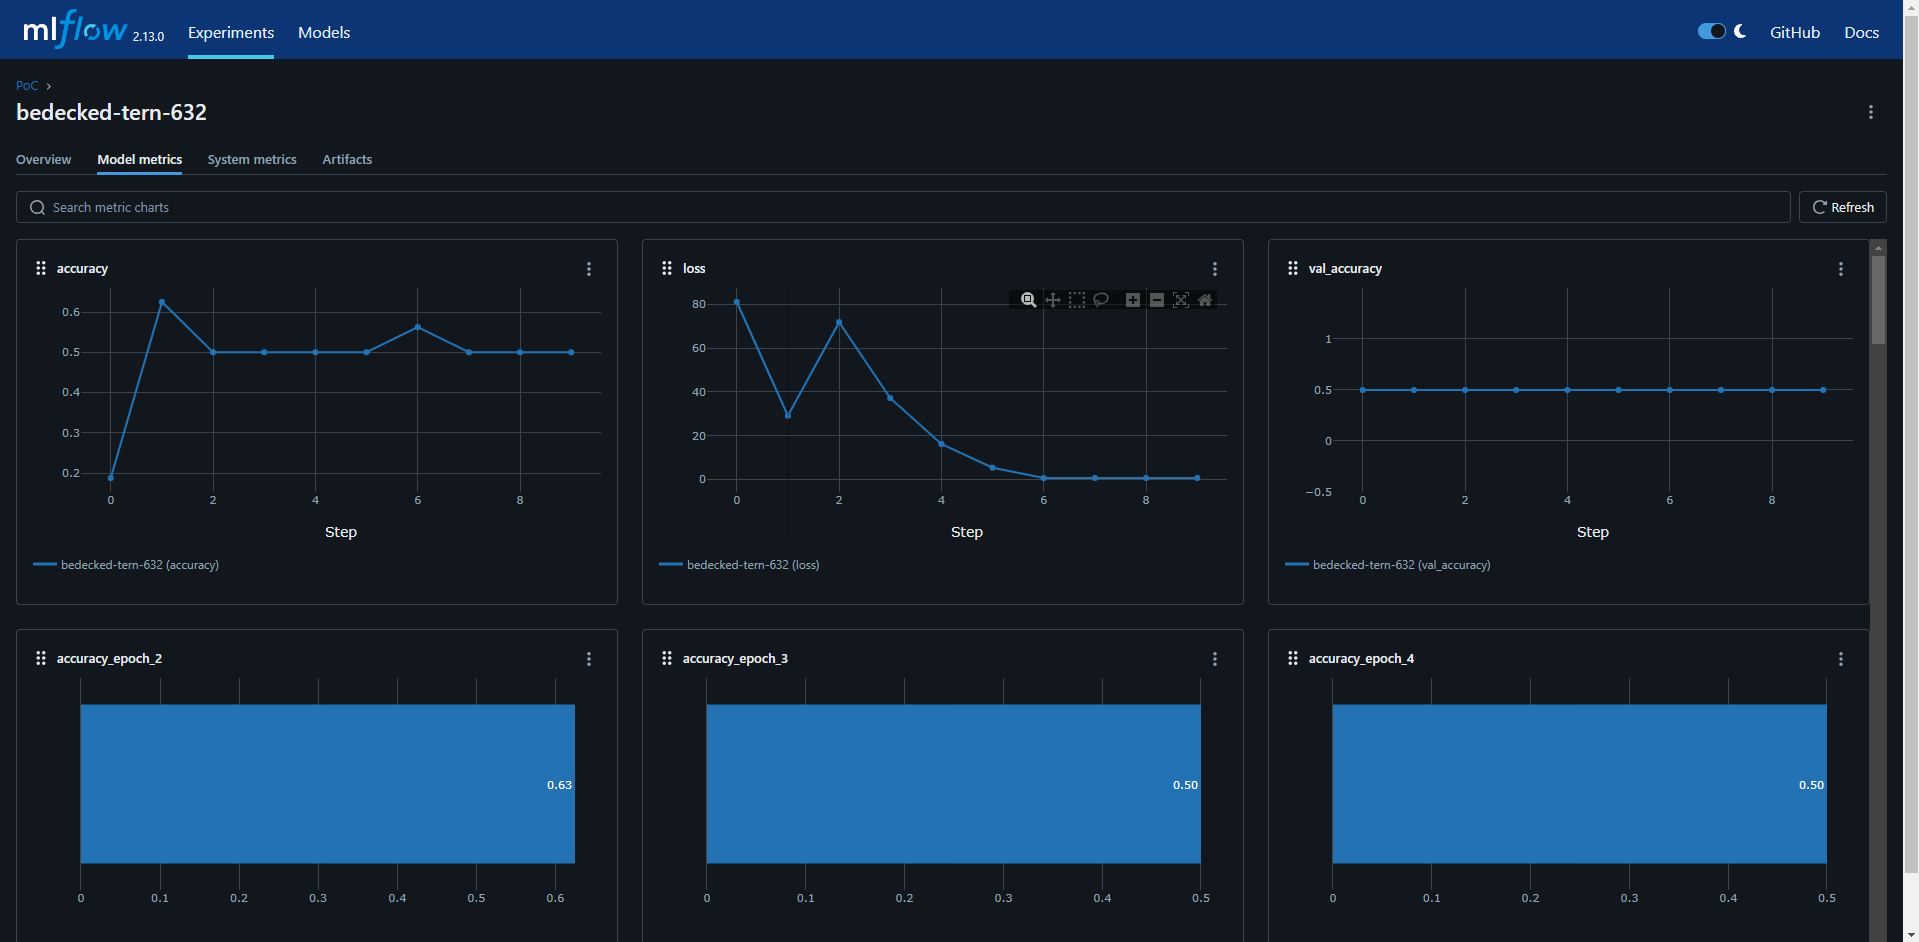
\includegraphics[width=1.0\linewidth]{graphics/mlflow_Graph.PNG}
  \captionof{figure}{Grafieken die de prestatie van de pipeline aantonen}
  \label{fig:mlflow_grafiek}
\end{center}

Figuur \ref{fig:mlflow_grafiek} toont de verschillende waarden die kunnen worden vastgesteld in MLflow. Op de afbeelding zijn de accuracy, loss, en validatie-accuracy van het model te zien, evenals de accuracy van enkele epochs tijdens het trainen van het model.
\section{Conclusies}

Proof of Concepts hebben de efficiëntie en bruikbaarheid van drie frameworks Prefect, ZenML en Dagster voor het lokaal uitvoeren van machine learning pipelines onderzocht. Deze analyse vormt de basis voor aanbevelingen over welk framework het meest geschikt is voor het opleidingsonderdeel Machine Learning Operations.

Prefect biedt een intuïtieve gebruikersinterface en uitgebreide functies voor workflowbeheer. Het heeft een eenvoudige installatie en configuratie, en integreert naadloos met MLFlow voor experiment tracking.

ZenML biedt een gestructureerde aanpak voor het ontwikkelen en uitvoeren van machine learning pipelines, met gebruik van decorators om Python-functies om te zetten naar ZenML-stappen. Enkele uitdagingen zijn de beperkte ondersteuning voor bepaalde datatypes en compatibiliteitsproblemen met oudere library-versies.

Dagster richt zich op data orchestration en biedt een krachtig platform voor het bouwen en uitvoeren van data pipelines. Het gebruikt een concept genaamd assets om taken te definiëren en te orchestreren, maar vereist een complexere configuratie dan de andere twee frameworks.

Prefect wordt aanbevolen voor het opleidingsonderdeel Machine Learning Operations vanwege de gebruiksvriendelijke interface, krachtige functies voor workflowbeheer en integratie met MLFlow. Het biedt een ideale balans tussen eenvoud, efficiëntie en functionaliteit, geschikt voor zowel educatieve als professionele toepassingen. Hierdoor kunnen studenten effectief machine learning pipelines ontwikkelen en beheren en zich voorbereiden op toekomstige uitdagingen in het werkveld.
\section{Toekomstig onderzoek}

In de toekomst kan er gekeken worden naar de impact van het lokaal uitvoeren van machine learning-pipelines. Dit kan eventueel verbeteringen voorstellen of bottlenecks identificeren met verschillende software- of hardwareoplossingen. Daarnaast kunnen ook andere manieren van het implementeren van de frameworks worden onderzocht, zoals met multithreading of andere technologieën.
\end{multicols}
\end{document}